\documentclass[11pt,a4paper]{article}
\usepackage[utf8]{inputenc}
\usepackage[T1]{fontenc}
\usepackage{amsmath,amssymb}
\usepackage[margin=2.5cm]{geometry}
\usepackage{tikz}
\usepackage{pgfplots}
\pgfplotsset{compat=1.18}
\usetikzlibrary{arrows.meta,positioning}
\usepackage{xcolor}

\newcommand{\sgn}{\operatorname{sgn}}

\setlength{\parindent}{0pt}
\setlength{\parskip}{6pt}

\begin{document}

\begin{center}
{\large Technical Neural Networks Assignment 1}\\[4pt]
{\bfseries Name: Mohamadhosein Sabaghi(50547423)}
\end{center}

\section*{Assignment 1}

\begin{enumerate}
  \item \textbf{A lot of simple, interconnected processing units (neurons).} Many
  simple units working in parallel, not one complex one.
  \item \textbf{Modifiable, plastic connections (synapses, synaptic weights).}
  Connections can change strength -- this is how learning happens.
  \item \textbf{Mapping from an input vector to a scalar output value.} Several inputs
  combined into one output.
  \item \textbf{Nonlinear transfer function.} Output isn't a linear function of the
  input, e.g.\ a threshold.
\end{enumerate}

\section*{Assignment 2}

\textbf{Transformer} / self-attention mechanism -- not mentioned in the lecture. I came
across it while reading up on large language models and image generation models in my
own time, and traced it back to the original paper.

Reference: Vaswani et al., \emph{``Attention Is All You Need''}, NeurIPS 2017.

\section*{Assignment 3}

\begin{itemize}
  \item \textbf{1940--1960, Beginning:} McCulloch-Pitts neuron and Hebbian learning
  proposed, leading up to Rosenblatt's Perceptron.
  \item \textbf{1960--1982, Quiet Years:} interest reduced after Minsky \& Papert
  showed the Perceptron can't solve problems like XOR.
  \item \textbf{1980--1990, Renaissance:} Hopfield networks and backpropagation
  discovered and multi-layer networks became trainable.
  \item \textbf{1990--1999, Consolidation:} neural networks became one of the normal ML
  tools, used in practice.
  \item \textbf{since 2000, 2nd start-up:} deep learning takes off because of big data
  and GPUs.
\end{itemize}

\section*{Assignment 4}

we know that a neuron sums the weighted inputs and fires if the sum is more than a threshold
$\Theta_m$:
\[
  \mathrm{net}^{*}_m = \sum_{n=1}^{N} w_{nm}x_n, \qquad
  y_m = 1 \text{ if } \mathrm{net}^{*}_m > \Theta_m, \text{ else } 0.
\]

Having a separate threshold for every neuron is very hard to handle and confusing. so we add one extra constant input $x_0=1$ with weight
$w_{0m}=-\Theta_m$:
\[
  \mathrm{net}_m = \sum_{n=0}^{N} w_{nm}x_n = \mathrm{net}^{*}_m - \Theta_m,
  \qquad y_m = 1 \text{ if } \mathrm{net}_m > 0.
\]

we call the constant input $x_0=1$ BIAS. Also $w_{0m}$ is the
BIAS-weight. It is just the negative threshold, added to the weights so it
can be learned the same as other weights.

For 2 inputs the decision line is $w_1x_1+w_2x_2+w_0=0$-- without $w_0$ this line would always go
through the origin, so $w_0$ is what lets it shift away from it.

\begin{center}
\begin{tikzpicture}[>=Stealth]
  \node (x0) at (0,1.6) {$x_0=1$};
  \node (x1) at (0,0) {$x_1$};
  \node (x2) at (0,-1.8) {$x_2$};
  \node[draw, circle] (sum) at (3,0) {$\Sigma$};
  \node[draw, rectangle, right=10mm of sum] (f) {$f$};
  \node[right=8mm of f] (y) {$y$};
  \draw[->] (x0) -- node[below,sloped,font=\small]{$w_0$} (sum);
  \draw[->] (x1) -- node[above,sloped,font=\small]{$w_1$} (sum);
  \draw[->] (x2) -- node[above,font=\small]{$w_2$} (sum);
  \draw[->] (sum) -- (f);
  \draw[->] (f) -- (y);
\end{tikzpicture}
\end{center}

\section*{Assignment 5}

both the points: $^3X$ and
$^4X$ sit right next to $(-1,3)$ but on opposite
sides of the line, so the line must pass exactly from $(-1,3)$. Same thing is for
$(5,-2)$ with $^7X,^8X$. So $g$ is the line through $(-1,3)$ and $(5,-2)$:
\[
  m=\frac{-2-3}{5-(-1)}=-\frac{5}{6}, \qquad
  x_2-3=-\tfrac56(x_1+1) \;\Rightarrow\; 5x_1+6x_2-13=0.
\]

if we test it on $^1X$ -> $(0,0;+1)$: $5(0)+6(0)-13=-13<0$, but $^1X$ should be $+1$, so we should change the
sign:
\[
  w_1=-5,\quad w_2=-6,\quad w_b=13, \qquad g:\; -5x_1-6x_2+13=0.
\]

\begin{center}
\begin{tabular}{c|c|c|c}
  & $(x_1,x_2)$ & $-5x_1-6x_2+13$ & $\hat y$ \\\hline
 $^1X$ & $(0,0)$ & $13$ & $+1$ \\
 $^2X$ & $(2,3)$ & $-15$ & $-1$ \\
 $^3X$ & $(-1-\varepsilon,3-\varepsilon)$ & $+11\varepsilon$ & $+1$ \\
 $^4X$ & $(-1+\varepsilon,3+\varepsilon)$ & $-11\varepsilon$ & $-1$ \\
 $^5X$ & $(-1,2)$ & $6$ & $+1$ \\
 $^6X$ & $(3,1)$ & $-8$ & $-1$ \\
 $^7X$ & $(5,-2+\varepsilon)$ & $-6\varepsilon$ & $-1$ \\
 $^8X$ & $(5-\varepsilon,-2)$ & $+5\varepsilon$ & $+1$ \\
\end{tabular}
\end{center}

\begin{center}
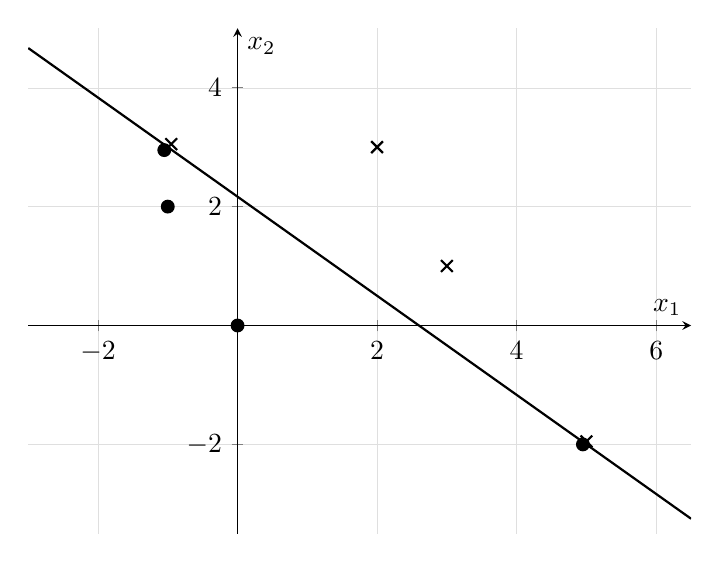
\begin{tikzpicture}
\begin{axis}[
    width=10cm, height=8cm,
    xlabel=$x_1$, ylabel=$x_2$,
    xmin=-3, xmax=6.5, ymin=-3.5, ymax=5,
    axis lines=middle,
    grid=both, grid style={line width=.1pt, draw=gray!25},
]
  \addplot[domain=-3:6.5, samples=2, thick] {(13-5*x)/6};
  \addplot[only marks, mark=*, mark size=2.3pt] coordinates {
    (0,0) (-1.05,2.95) (-1,2) (4.95,-2)
  };
  \addplot[only marks, mark=x, mark size=3pt, thick] coordinates {
    (2,3) (-0.95,3.05) (3,1) (5,-1.95)
  };
\end{axis}
\end{tikzpicture}
\end{center}

\section*{Assignment 6}

\textbf{AI use:} I used Claude to get help for this question. I gave it the assignment text directly and asked it to find
weights for single threshold neurons solving AND, NAND, NOR and to check
them against the truth tables. The weights it gave worked on the first try, so I didn't need to ask it for changes.

Single threshold neuron, $y=1$ if $w_1x_1+w_2x_2>\Theta$, else $0$:

\begin{center}
\begin{tabular}{l c c c}
 & $w_1$ & $w_2$ & $\Theta$ \\\hline
 AND  & $1$  & $1$  & $1.5$ \\
 NAND & $-1$ & $-1$ & $-1.5$ \\
 NOR  & $-1$ & $-1$ & $-0.5$ \\
\end{tabular}
\end{center}

\begin{tabular}{cc|cc|cc|cc}
 $x_1$&$x_2$ & \multicolumn{2}{c|}{AND} & \multicolumn{2}{c|}{NAND} & \multicolumn{2}{c}{NOR}\\
 & & net & $y$ & net & $y$ & net & $y$\\\hline
 0&0 & 0 & 0 & 0  & 1 & 0  & 1\\
 0&1 & 1 & 0 & $-1$ & 1 & $-1$ & 0\\
 1&0 & 1 & 0 & $-1$ & 1 & $-1$ & 0\\
 1&1 & 2 & 1 & $-2$ & 0 & $-2$ & 0\\
\end{tabular}

All three match the truth tables.

\begin{center}
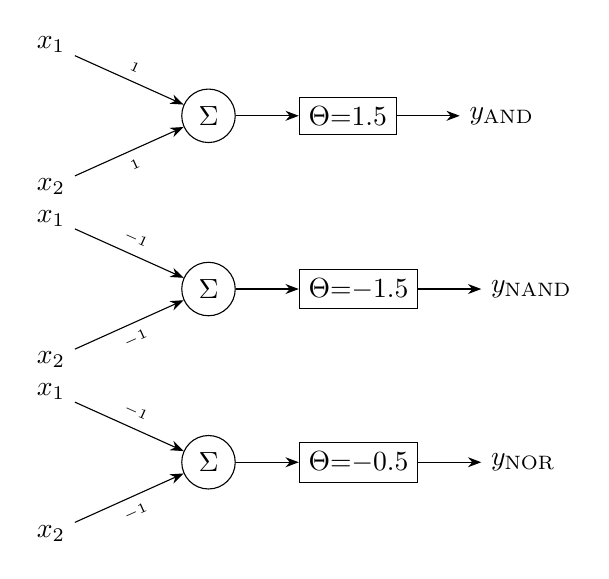
\begin{tikzpicture}[>=Stealth]
 \begin{scope}
   \node (x1) at (0,0.9) {$x_1$};
   \node (x2) at (0,-0.9) {$x_2$};
   \node[draw, circle] (sum) at (2,0) {$\Sigma$};
   \node[draw, rectangle, right=8mm of sum] (f) {$\Theta{=}1.5$};
   \node[right=8mm of f] (y) {$y_{\text{AND}}$};
   \draw[->] (x1) -- node[above,sloped,font=\tiny]{1} (sum);
   \draw[->] (x2) -- node[below,sloped,font=\tiny]{1} (sum);
   \draw[->] (sum) -- (f); \draw[->] (f) -- (y);
 \end{scope}
 \begin{scope}[yshift=-2.2cm]
   \node (x1) at (0,0.9) {$x_1$};
   \node (x2) at (0,-0.9) {$x_2$};
   \node[draw, circle] (sum) at (2,0) {$\Sigma$};
   \node[draw, rectangle, right=8mm of sum] (f) {$\Theta{=}{-}1.5$};
   \node[right=8mm of f] (y) {$y_{\text{NAND}}$};
   \draw[->] (x1) -- node[above,sloped,font=\tiny]{$-1$} (sum);
   \draw[->] (x2) -- node[below,sloped,font=\tiny]{$-1$} (sum);
   \draw[->] (sum) -- (f); \draw[->] (f) -- (y);
 \end{scope}
 \begin{scope}[yshift=-4.4cm]
   \node (x1) at (0,0.9) {$x_1$};
   \node (x2) at (0,-0.9) {$x_2$};
   \node[draw, circle] (sum) at (2,0) {$\Sigma$};
   \node[draw, rectangle, right=8mm of sum] (f) {$\Theta{=}{-}0.5$};
   \node[right=8mm of f] (y) {$y_{\text{NOR}}$};
   \draw[->] (x1) -- node[above,sloped,font=\tiny]{$-1$} (sum);
   \draw[->] (x2) -- node[below,sloped,font=\tiny]{$-1$} (sum);
   \draw[->] (sum) -- (f); \draw[->] (f) -- (y);
 \end{scope}
\end{tikzpicture}
\end{center}

\end{document}
